\begin{frame}{Metodología}
\begin{figure}[h]
	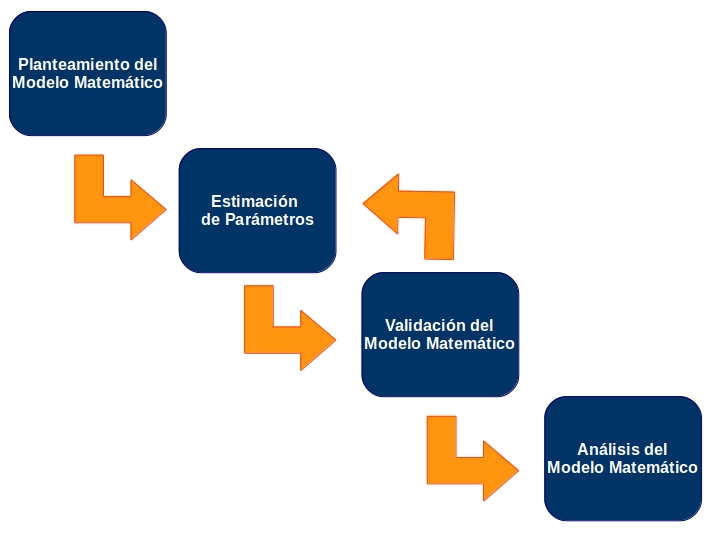
\includegraphics[width=\textwidth]{FLOWCHART}
\end{figure}
\end{frame}


\begin{frame}{Descripción del Modelo Matemático}

\begin{columns}
	\begin{column}{0.4\textwidth}
		\begin{figure}[h]
			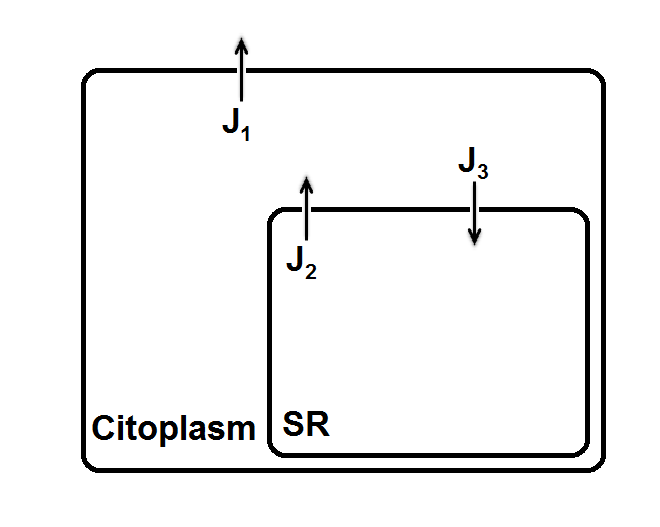
\includegraphics[width=1.1\textwidth]{Flujos}
		\end{figure}
	\end{column}
	\begin{column}{0.6\textwidth}
	\Large	\begin{eqnarray*}
		\frac{d[Ca^{2+}]_{i}^{T}}{dt} & = & -J_{1} + J_{2} - J_{3} \\
		\frac{d[Ca^{2+}]_{SR}^{T}}{dt} & = & \frac{J_{3} - J_{2}}{\gamma}
		\end{eqnarray*}
	\end{column}
	 \blfootnote{{\tiny Norma Citlalcue Pérez Rosas. Análisis de la dinámica del ion calcio durante su liberación por
	 	medio de los receptores de rianodina : un enfoque de modelación matemática. Thesis, Centro de
	 	Investigación y de Estudios Avanzados del Instituto Politécnico Nacional, 2016.}}
\end{columns}

\end{frame}

\begin{frame}{Descripción del Modelo Matemático}
	\Large \begin{center}
		\textbf{Flujo a Través de los Mecanismos de Remoción de la Membrana Plasmática}
	\end{center}
	
	\begin{equation*}
	J_1 = a\left[[Ca^{2+}]_i - [\overline{Ca^{2+}}]_i\right]
	\end{equation*}	
	\begin{align*}
	a & \rightarrow \text{Tasa de remoción de calcio}  \\
	[Ca^{2+}]_i & \rightarrow \text{Concentración de calcio libre en citoplasma} \\
	[\overline{Ca^{2+}}]_i & \rightarrow \text{Concentración basal de calcio en citoplasma}
	\end{align*}

\end{frame}

\begin{frame}{Descripción del Modelo Matemático}
	\Large \begin{center}
			\textbf{Flujo a Través de los RyR}
	\end{center}	
	\begin{equation*}
		J_2 = b\gamma^{n_v}f\left([Ca^{2+}]_i,[Caff]\right)\left[[Ca^{2+}]_{SR}-[Ca^{2+}]_i\right]
	\end{equation*}
	\begin{align*}
	b & \rightarrow \text{Flujo máximo} \\
	\gamma & \rightarrow \text{Vol retículo:Vol célula} \\
	n_v & \rightarrow \text{Dimensión fractal del retículo} \\
	f\left([Ca^{2+}]_i,[Caff]\right) & \rightarrow \text{Frecuencia de apertura de un RyR} \\
	[Ca^{2+}]_{SR} & \rightarrow \text{Concentración calcio libre luminal}
	\end{align*}
	
\end{frame}

\begin{frame}{Descripción del Modelo Matemático}
	\Large \begin{center}
		\textbf{Flujo a Través de la bomba SERCA}
	\end{center}
	
	\begin{equation*}
		J_3 = c\frac{[Ca^{2+}]^{n_s}_i}{K^{n_s}_s+[Ca^{2+}]^{n_s}_i}
	\end{equation*}
	\begin{align*}
	c & \rightarrow \text{Flujo máximo}  \\
	[Ca^{2+}]_i & \rightarrow \text{Concentración de calcio libre en citoplasma} \\
	K_s & \rightarrow \text{Constante de saturación media} \\
	n_s & \rightarrow \text{Coeficiente de Hill}
	\end{align*}
\end{frame}

\begin{frame}{Descripción del Modelo Matemático}
	\begin{center}
		{\Large \textbf{Capacidad Amortiguadora del los Compartimentos Celulares}}
	\end{center}
	
	\large \begin{columns}
		\begin{column}{0.45\textwidth}
			\textbf{Citoplasma}
			\begin{equation*}
			\Delta [Ca^{2+}]_i = \frac{\Delta [Ca^{2+}]_i^T}{\beta}
			\end{equation*}
			\begin{align*}
			\beta & \rightarrow \text{Capacidad amortiguadora} \\
			[Ca^{2+}]_i & \rightarrow \text{Calcio libre} \\
			[Ca^{2+}]_i^T & \rightarrow \text{Calcio total}
			\end{align*}
		\end{column}
		\begin{column}{0.55\textwidth}
			\textbf{Retículo Sarcoplásmico}
			\begin{equation*}
			[Ca^{2+}]_{SR} = [Ca^{2+}]_{SR}^T - [Ca^{2+}]_{SR}^B 
			\end{equation*}
			\begin{align*}
			[Ca^{2+}]_{SR} & \rightarrow \text{Calcio libre} \\
			[Ca^{2+}]_{SR}^T & \rightarrow \text{Calcio total} \\
			[Ca^{2+}]_{SR}^B & \rightarrow \text{Calcio unido}
			\end{align*}
		\end{column}
	\end{columns}	
\end{frame}